\documentclass[twoside]{article}
\input{ISC18-english.sty}
%%%%%%%%%%%%%%%%%%%%%%%%%%%%  Make sure to compile twice for proper cross-references. %%%%%%%%%%%%%%%%%%%%%%%
%%%%%%% For proper display of references, compile the document twice. %%%%%%%%%%%%%%%%%%%%% 
\usepackage{amsmath, amssymb, bm,  amsfonts}
\usepackage{graphicx}
\usepackage{booktabs}
\usepackage{multirow}
\usepackage{hyperref}
\usepackage{algorithmic}
\usepackage{array}
\usepackage{caption}
\usepackage{subfigure}
%%%%%%%%%%%%%%% If using TeX Live, compile using pdflatex command %%%%%%%%%%%%%%%%%%%%%%%
\begin{document}
\thispagestyle{empty}
%%%%%%%%%%%%%%%%% Article title header  %%%%%%%%%%%%%%%%%%%%
\fancyhead[LE]{Synthetic Medical Data Generation in Pediatric Osteopenia}
%%%%%%%%%%%%%%%%% Article authors header   %%%%%%%%%%%%%%%%%%%%
\fancyhead[RO]{R.Yousefi, M.Attarhoseini}
\begin{center}
{
\includegraphics [height=25mm, width=150.3mm] {Images/isc18E}} \\
\vspace*{-1.8cm}
%\begin{center}
%\color{blue} 
%{\hspace{0.1cm}\rule{\textwidth}{1mm}}\\
%\end{center}
\vspace*{4cm}
%%%%%%%%%%%%%%%%% Article title  %%%%%%%%%%%%%%%%%%%%
{\Large \bf Comparative Evaluation of Synthetic Medical Data Generation Methods in Pediatric Osteopenia}\\
%%%%%%%%%%%%%%%%% Article authors and affiliations %%%%%%%%%%%%%%%%%%%%
{\bf
Razieh Yousefi  \footnote[1]{{\bf Corresponding Author:} {\tt raziehyousefi87@gmail.com }}, Maryam Attarhoseini$^2$ \\
$^1$Ph.D. in Biostatistics, Faculty of Health, Mashhad University of Medical Sciences, Mashhad, Iran \\
$^2$Pediatric Endocrinologist, Faculty of Medicine, Mashhad University of Medical Sciences, Mashhad, Iran }
\end{center}
\rule{\textwidth}{0.2mm}\\
%%%%%%%%%%%%%%%%% Article abstract  %%%%%%%%%%%%%%%%%%%%
\noindent{\bf Abstract:}\\
Medical datasets, often suffer from limited sample sizes. Synthetic data generation may support data augmentation, privacy-preserving sharing, and methodological validation. This study compared six synthetic data generation strategies using a pediatric osteopenia dataset ($n=71$) from children with type 1 diabetes mellitus, including conditional and non-conditional Bootstrap, Multivariate Normal (MVN), and Gaussian Copula methods.
Synthetic datasets of 500 samples were evaluated using utility (TSTR ROC analysis), fidelity (Kolmogorov--Smirnov testing and correlation preservation), and privacy (Nearest Neighbor Distance Ratio; NNDR) assessments. The real-data model achieved an AUC of $0.796$. Conditional Bootstrap ($AUC = 0.786$), conditional MVN ($AUC = 0.776$), and conditional Copula ($AUC = 0.776$) preserved predictive performance well, whereas the non-conditional Copula approach performed poorly ($AUC = 0.224$, $p = 0.011$).
Bootstrap and Copula methods showed strong distributional similarity, while conditional MVN demonstrated the best correlation preservation. Privacy analysis indicated high disclosure risk for Bootstrap methods, whereas MVN and Copula approaches provided substantially better privacy protection. Overall, conditional MVN provided the best balance between utility, fidelity, and privacy preservation in this low-sample clinical setting.


\noindent{\bf Keywords:}
Synthetic data, Multivariate normal, Gaussian copula, Bootstrap, Pediatric osteopenia

\noindent{\bf Mathematics Subject Classification (2010):} $\rm 62H12$, $\rm 62P10$, $\rm 68T07$.\\
\hspace{1cm}\rule{\textwidth}{0.2mm}

%%%%%%%%%%%%%%%%%%%%%%%%%%%%%%%%%%%%%%%%%%%%%%%%%%%%%%%%%%%%%%%%%%%%%%%%%%%%%%%%%%%%%%%%%%%%%%%%%%%%%%%%

%============================================================
\section{Introduction}

\noindent The increasing use of machine learning and statistical modeling in medicine has created substantial demand for high-quality clinical datasets. However, medical datasets are frequently limited by small sample sizes, especially in rare diseases, and specialized clinical settings like pediatric populations. Ethical restrictions, patient privacy regulations, and the high cost of clinical data acquisition further complicate data sharing and methodological reproducibility \cite{gonzales2023synthetic}.

\noindent Synthetic data generation has emerged as a promising strategy for addressing these challenges. By generating artificial observations that preserve the statistical properties of real datasets, synthetic data can support data augmentation, privacy-preserving data sharing, external validation, and methodological benchmarking without directly exposing sensitive patient information \cite{mendes2025synthetic}.

\noindent Several approaches have been proposed for synthetic medical data generation, including classical statistical methods such as multivariate normal simulation and copula-based modeling \cite{jeong2016copula}, as well as deep learning frameworks including GANs and VAEs \cite{endres2022synthetic}. While deep learning methods often require large datasets and may perform poorly in low-sample settings, simpler statistical approaches are generally more robust and interpretable for small medical datasets. In addition, synthetic generation can be performed using either non-conditional methods, which model the overall joint distribution, or conditional methods, which separately model outcome classes to better preserve clinically relevant predictor–outcome relationships.

\noindent Therefore, this study aimed to systematically compare conditional and non-conditional synthetic data generation approaches in a small pediatric clinical dataset.

%============================================================
\section{Materials and Methods}

\subsection{Real Dataset}

\noindent \noindent The study dataset consisted of 71 pediatric patients with type 1 diabetes who were evaluated for osteopenia at a tertiary pediatric endocrinology clinic after preprocessing and removal of incomplete observations. Patients were aged 7--18 years, had disease duration greater than two years, and were receiving insulin therapy. Osteopenia prevalence was 33.8\%. The dataset included five continuous clinical variables: 25-hydroxyvitamin D, age, body mass index, serum calcium, and glycated hemoglobin (HBA1C), along with two categorical variables: gender and vitamin D supplementation status. Variables were selected based on univariate statistical significance and/or clinical relevance according to expert opinion.



\subsection{Train-Test Splitting}

\noindent To evaluate predictive utility under realistic external validation conditions, the dataset was randomly divided into training (70\%) and testing (30\%) subsets using stratified sampling to preserve osteopenia prevalence.

\subsection{Reference Predictive Model}

\noindent A logistic regression model was trained on the real training dataset. Predictive discrimination was evaluated using the area under the receiver operating characteristic curve (AUC).

\subsection{Synthetic Data Generation Methods}

\noindent Six synthetic data generation strategies were evaluated:

\textbf{Non-Conditional Bootstrap} Synthetic observations were generated by random sampling with replacement from the original training dataset.

\textbf{Conditional Bootstrap} Bootstrap sampling was performed separately within osteopenia classes to preserve outcome-specific relationships.

\textbf{Non-Conditional MVN} Continuous variables were generated from a multivariate normal distribution:
\[
\mathbf{X}_{\mathrm{synth}}
\sim
\mathcal{N}
\left(
\boldsymbol{\mu},
\boldsymbol{\Sigma}
\right)
\]

\noindent where $\boldsymbol{\mu}$ and $\boldsymbol{\Sigma}$ were estimated from the entire training dataset.

\textbf{Conditional MVN} Separate multivariate normal distributions were estimated for each osteopenia class:
\[
\mathbf{X}_{\mathrm{synth}}^{(g)}
\sim
\mathcal{N}
\left(
\boldsymbol{\mu}_g,
\boldsymbol{\Sigma}_g
\right)
\]

\noindent where $g \in {0,1}$ represents osteopenia status.

\textbf{Non-Conditional Gaussian Copula} Dependence structure was modeled using a Gaussian copula fitted to the entire dataset:
\[
C_{\mathbf{P}}(\mathbf{u}) =
\Phi_{\mathbf{P}}
\left(
\Phi^{-1}(u_1), \ldots, \Phi^{-1}(u_d)
\right)
\]

\textbf{Conditional Gaussian Copula} Separate Gaussian copula models were estimated within each osteopenia class to preserve conditional dependence structures.

\subsection{Validation Framework}

\subsubsection{Utility Assessment}

\noindent Utility was evaluated using a Train-on-Synthetic Test-on-Real (TSTR) framework. LR models were trained on each synthetic dataset and evaluated on the held-out real testing set. Utility metrics included: AUC, Brier score, DeLong statistical comparison against the real ROC curve, and Utility Ratio as \cite{hernandez2025comprehensive}:
\[
\text{Utility Ratio} =
\frac{\text{Synthetic AUC}}
{\text{Real AUC}}
\]

\subsubsection{Fidelity Assessment}

\noindent Fidelity was evaluated using Kolmogorov--Smirnov (KS) tests for marginal distribution similarity, and correlation preservation measured by mean absolute correlation difference relative to the real dataset \cite{hernandez2025comprehensive}.

\subsubsection{Privacy Assessment}

\noindent Privacy protection was evaluated using the Nearest Neighbor Distance Ratio (NNDR). Higher NNDR values indicate lower disclosure risk \cite{hernandez2025comprehensive}:
\[
\text{NNDR} =
\frac{
\text{Mean nearest synthetic-to-real distance}
}{
\text{Mean nearest real-to-real distance}
}
\]

%============================================================
\section{Results}

\paragraph {Reference Model Performance} The logistic regression model trained on the real dataset achieved an AUC of 0.796 (95\% CI: 0.575--1.000).The relatively wide confidence intervals likely reflect the limited sample size and class imbalance of the pediatric dataset.

\paragraph {Utility Assessment} As we see in Table~\ref{tab:utility} Conditional methods consistently outperformed their non-conditional counterparts. The conditional Bootstrap method achieved the highest utility preservation with an AUC of 0.786 and Utility Ratio of 0.987. Conditional MVN and conditional Copula methods also demonstrated strong predictive performance, each achieving an AUC of 0.776. In contrast, the non-conditional Copula method demonstrated severe utility degradation (AUC = 0.224), indicating failure to preserve clinically relevant predictor-outcome relationships when outcome conditioning was omitted.

\begin{table}[htbp]
\scriptsize
\centering
\caption{Comparative validation results}
\begin{tabular}{lcccccc}
\toprule
\textbf{Method} & \textbf{AUC} & \textbf{CI Lower} & \textbf{CI Upper} & \textbf{Brier} & \textbf{Utility Ratio} & \textbf{p-value} \\
\midrule
\textbf{Boot\_NC} & 0.786 & 0.555 & 1.000 & 0.195 & 0.987 & 0.8322 \\
\textbf{MVR\_NC}  & 0.612 & 0.359 & 0.866 & 0.218 & 0.769 & 0.2688 \\
\textbf{Cop\_NC}  & 0.224 & 0.000 & 0.469 & 0.252 & 0.282 & 0.0107 \\
\textbf{Boot\_C}  & 0.786 & 0.549 & 1.000 & 0.178 & 0.987 & 0.7993 \\
\textbf{MVR\_C}   & 0.776 & 0.534 & 1.000 & 0.185 & 0.974 & 0.6659 \\
\textbf{Cop\_C}   & 0.776 & 0.534 & 1.000 & 0.181 & 0.974 & 0.6490 \\
\bottomrule
\end{tabular}
\label{tab:utility}
\end{table}

\paragraph{Fidelity Assessment} KS testing demonstrated good distribution preservation across methods, particularly for Bootstrap and Copula approaches, with most p-values exceeding 0.90. Conditional MVN generation showed slightly larger but still acceptable deviations from the real distributions.

\paragraph{Correlation Preservation}
\noindent As we see in Table \ref{tab:correlation}, the conditional MVR method demonstrated the lowest mean absolute correlation difference (0.018), indicating superior preservation of the original multivariate dependency structure. The non-conditional bootstrap, non-conditional MVR, non-conditional Copula, and conditional Copula methods showed slightly larger deviations, though all remained within acceptable ranges (0.030–0.041).

\paragraph{Privacy Assessment}
\noindent Bootstrap methods demonstrated essentially no privacy protection because synthetic observations were direct resamples of real patients. In contrast, MVN and Copula approaches produced substantially improved privacy protection with NNDR values near or above 1 (Table \ref{tab:privacy}).

\begin{table}[htb]
\centering

\begin{minipage}{0.48\textwidth}
\centering
\scriptsize
\caption{Correlation Preservation Results}
\begin{tabular}{lc}
\toprule
\textbf{Method} & \textbf{Mean Absolute Correlation Difference} \\
\midrule
Boot\_NC & 0.030 \\
MVR\_NC & 0.040 \\
Cop\_NC & 0.038 \\
Boot\_C & 0.041 \\
MVR\_C & 0.018 \\
Cop\_C & 0.041 \\

\bottomrule
\end{tabular}
\label{tab:correlation}
\end{minipage}
\hfill
\begin{minipage}{0.48\textwidth}
\centering
\scriptsize
\caption{Privacy Assessment Using NNDR}
\begin{tabular}{lc}
\toprule
\textbf{Method} & \textbf{NNDR} \\
\midrule
Boot\_NC & 0.000 \\
MVR\_NC & 1.135 \\
Cop\_NC & 0.958 \\
Boot\_C & 0.000 \\
MVR\_C & 1.037 \\
Cop\_C & 0.924 \\
\bottomrule
\end{tabular}
\label{tab:privacy}
\end{minipage}

\end{table}


\paragraph{ROC Curve Comparison}

\noindent Figure \ref{ROC} compares the ROC curves of predictive models trained on real and synthetic datasets. The conditional MVR and conditional Copula methods achieved ROC curves closely approximating the real-data model, whereas the non-conditional Copula approach demonstrated substantially degraded discrimination performance.

\noindent The ROC analysis confirmed that conditional synthetic generation substantially improved predictive utility compared with non-conditional approaches. In particular, the conditional MVR method achieved an AUC of 0.776 with a utility ratio of 0.974, closely approximating the real-data reference model (AUC = 0.796).

\begin{figure}[htbp]
\centering
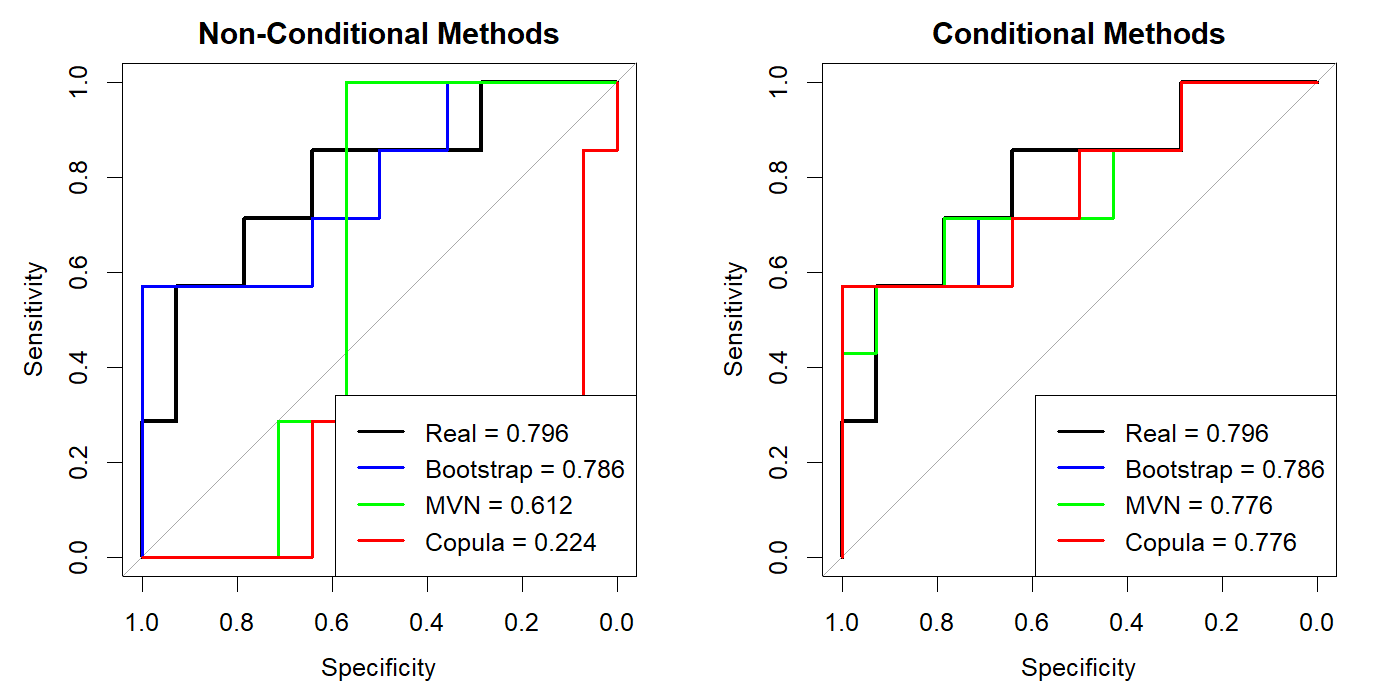
\includegraphics[width=0.6\linewidth]{Images/ROC.png}
\caption{ROC curve comparison between the real-data model and synthetic-data-trained models for conditional and non-conditional synthetic generation methods.}
\label{ROC}
\end{figure}

%============================================================
\section{Discussion}
\noindent This study provides a comparative evaluation of conditional and non-conditional synthetic medical data generation methods in a low-sample pediatric clinical dataset. Overall, conditional generation substantially improved predictive utility across both MVN and Copula frameworks, highlighting the importance of preserving outcome-specific dependency structures during synthetic data generation.

 \noindent Previous studies have reported that conditional distribution modeling may outperform joint MVN approaches when multivariate normality assumptions are violated, although joint MVN models remain appropriate when variables are approximately normally distributed \cite{smania2021conditional}. While theoretical work suggests that conditional and unconditional formulations can be asymptotically equivalent under certain settings \cite{bucher2019note}, our findings indicate that conditioning has important practical implications in small clinical datasets.

\noindent In particular, the markedly poor performance of the non-conditional Copula approach suggests that clinically meaningful predictor--outcome relationships were not adequately preserved. Conditional copula models are especially important when dependence structures vary according to clinical outcomes or covariates \cite{acar2013statistical}. Without conditioning on the outcome variable, synthetic generation may distort associations that are essential for downstream predictive modeling.

\noindent Bootstrap methods achieved the highest predictive utility because they directly resampled real observations. However, this resulted in essentially no privacy protection, limiting their suitability for privacy-sensitive data sharing applications. In contrast, MVN and Copula approaches generated more distinct synthetic observations while maintaining acceptable predictive performance, thereby providing a more balanced tradeoff between utility and privacy preservation.
\noindent Among all evaluated approaches, conditional MVN generation achieved the best overall balance between predictive utility, fidelity, and privacy protection. Several factors may explain this finding. First, the continuous clinical variables were approximately normally distributed, making MVN assumptions suitable for the dataset. Second, simpler parametric models may be more stable and less prone to overfitting in very small samples. Third, conditional modeling preserved clinically meaningful covariance structures while maintaining outcome-specific relationships. 
\noindent Furthermore, conditional MVN generation demonstrated the best correlation preservation, indicating superior maintenance of multivariable dependency patterns relative to the alternative methods. These findings suggest that conditional MVN simulation may provide a practical compromise between statistical realism, predictive performance, and disclosure protection in low-sample clinical settings.

\noindent Several practical implications emerge from these results. First, conditional synthetic generation should generally be preferred over non-conditional approaches in predictive clinical applications. Second, evaluation of synthetic data should incorporate utility, fidelity, and privacy assessments rather than relying on a single performance metric. Finally, the results demonstrate that classical statistical approaches, particularly conditional MVN simulation, remain highly effective and computationally efficient alternatives to more complex generative frameworks in low-resource medical settings.

\noindent Despite these encouraging findings, several limitations should be acknowledged. The analysis was based on a single small pediatric dataset, which may limit generalizability. Advanced deep learning approaches such as GANs and VAEs were not evaluated because they typically require substantially larger datasets. In addition, categorical predictors were generated using empirical resampling rather than explicit joint modeling, which may not fully preserve categorical dependencies. Finally, utility assessment was limited to logistic regression and may differ with other machine learning algorithms.
\noindent Future studies should validate these findings across larger and more diverse clinical cohorts, evaluate additional predictive models, and compare classical statistical approaches with modern deep generative frameworks under varying sample-size conditions.


%============================================================
\section{Conclusion}

\noindent This study demonstrates that conditional synthetic data generation substantially improves predictive utility compared with non-conditional approaches in small medical datasets. Among the evaluated methods, conditional MVN generation provided the best overall balance between predictive utility, structural fidelity, and privacy protection. Bootstrap methods achieved excellent predictive utility but failed to provide adequate privacy protection.These findings support the use of conditional MVN generation for privacy-preserving synthetic medical data generation in low-resource clinical settings.
% ============================================================
% REFERENCES
% ============================================================
\begin{thebibliography}{9}

%%%%%%%%%%%%%%%%%%%%%%%%%%%%%%%%%%%%%%%%
\bibitem[Gonzales et al.(2023)]{gonzales2023synthetic}
A. Gonzales, G. Guruswamy, and S. R. Smith, ``Synthetic data in health care: A narrative review,'' \textit{PLOS Digital Health}, vol. 2, no. 1, p. e0000082, 2023.

\bibitem[Mendes et al.(2025)]{mendes2025synthetic}
J. M. Mendes, A. Barbar, and M. Refaie, ``Synthetic data generation: A privacy-preserving approach to accelerate rare disease research,'' \textit{Frontiers in Digital Health}, vol. 7, p. 1563991, 2025.

\bibitem[Jeong et al.(2016)]{jeong2016copula}
B. Jeong, W. Lee, D.-S. Kim, and H. Shin, ``Copula-based approach to synthetic population generation,'' \textit{PLOS ONE}, vol. 11, no. 8, p. e0159496, 2016.

\bibitem[Marin(2022)]{marin2022evaluating}
J. Marin, ``Evaluating synthetically generated data from small sample sizes: An experimental study,'' \textit{arXiv e-prints}, pp. arXiv--2211, 2022.

\bibitem[Endres et al.(2022)]{endres2022synthetic}
M. Endres, A. Mannarapotta Venugopal, and T. S. Tran, ``Synthetic data generation: A comparative study,'' in \textit{Proceedings of the 26th International Database Engineered Applications Symposium}, pp. 94--102, 2022.

\bibitem[Hernandez et al.(2025)]{hernandez2025comprehensive}
M. Hernandez, P. A. Osorio-Marulanda, M. Catalina, L. Loinaz, G. Epelde, and N. Aginako, ``Comprehensive evaluation framework for synthetic tabular data in health: Fidelity, utility and privacy analysis of generative models with and without privacy guarantees,'' \textit{Frontiers in Digital Health}, vol. 7, p. 1576290, 2025.

\bibitem[Smania and Jonsson(2021)]{smania2021conditional}
G. Smania and E. N. Jonsson, ``Conditional distribution modeling as an alternative method for covariates simulation: Comparison with joint multivariate normal and bootstrap techniques,'' \textit{CPT: Pharmacometrics \& Systems Pharmacology}, vol. 10, no. 4, pp. 330--339, 2021.


\bibitem[B{\"u}cher and Kojadinovic(2019)]{bucher2019note}
A. B{\"u}cher and I. Kojadinovic, ``A note on conditional versus joint unconditional weak convergence in bootstrap consistency results,'' \textit{Journal of Theoretical Probability}, vol. 32, no. 3, pp. 1145--1165, 2019.


\bibitem[Acar et al.(2013)]{acar2013statistical}
E. F. Acar, R. V. Craiu, and F. Yao, ``Statistical testing of covariate effects in conditional copula models,'' 2013.



\end{thebibliography}
 \end{document}

